% Options for packages loaded elsewhere
\PassOptionsToPackage{unicode,linktoc=all}{hyperref}
\PassOptionsToPackage{hyphens}{url}
\PassOptionsToPackage{dvipsnames,svgnames,x11names}{xcolor}
%
\documentclass[
  a4paper,
]{article}
\usepackage{amsmath,amssymb}
\usepackage{lmodern}
\usepackage{iftex}
\ifPDFTeX
  \usepackage[T1]{fontenc}
  \usepackage[utf8]{inputenc}
  \usepackage{textcomp} % provide euro and other symbols
\else % if luatex or xetex
  \usepackage{unicode-math}
  \defaultfontfeatures{Scale=MatchLowercase}
  \defaultfontfeatures[\rmfamily]{Ligatures=TeX,Scale=1}
\fi
% Use upquote if available, for straight quotes in verbatim environments
\IfFileExists{upquote.sty}{\usepackage{upquote}}{}
\IfFileExists{microtype.sty}{% use microtype if available
  \usepackage[]{microtype}
  \UseMicrotypeSet[protrusion]{basicmath} % disable protrusion for tt fonts
}{}
\makeatletter
\@ifundefined{KOMAClassName}{% if non-KOMA class
  \IfFileExists{parskip.sty}{%
    \usepackage{parskip}
  }{% else
    \setlength{\parindent}{0pt}
    \setlength{\parskip}{6pt plus 2pt minus 1pt}}
}{% if KOMA class
  \KOMAoptions{parskip=half}}
\makeatother
\usepackage{xcolor}
\IfFileExists{xurl.sty}{\usepackage{xurl}}{} % add URL line breaks if available
\IfFileExists{bookmark.sty}{\usepackage{bookmark}}{\usepackage{hyperref}}
\hypersetup{
  pdftitle={The Secret Trapdoor to Success},
  pdfauthor={R (Chandra) Chandrasekhar},
  pdflang={en-GB},
  colorlinks=true,
  linkcolor={DarkOliveGreen},
  filecolor={Purple},
  citecolor={DarkKhaki},
  urlcolor={Maroon},
  pdfcreator={LaTeX via pandoc}}
\urlstyle{same} % disable monospaced font for URLs
\usepackage[margin=25mm]{geometry}
\usepackage{longtable,booktabs,array}
\usepackage{calc} % for calculating minipage widths
% Correct order of tables after \paragraph or \subparagraph
\usepackage{etoolbox}
\makeatletter
\patchcmd\longtable{\par}{\if@noskipsec\mbox{}\fi\par}{}{}
\makeatother
% Allow footnotes in longtable head/foot
\IfFileExists{footnotehyper.sty}{\usepackage{footnotehyper}}{\usepackage{footnote}}
\makesavenoteenv{longtable}
\usepackage{graphicx}
\makeatletter
\def\maxwidth{\ifdim\Gin@nat@width>\linewidth\linewidth\else\Gin@nat@width\fi}
\def\maxheight{\ifdim\Gin@nat@height>\textheight\textheight\else\Gin@nat@height\fi}
\makeatother
% Scale images if necessary, so that they will not overflow the page
% margins by default, and it is still possible to overwrite the defaults
% using explicit options in \includegraphics[width, height, ...]{}
\setkeys{Gin}{width=\maxwidth,height=\maxheight,keepaspectratio}
% Set default figure placement to htbp
\makeatletter
\def\fps@figure{htbp}
\makeatother
\setlength{\emergencystretch}{3em} % prevent overfull lines
\providecommand{\tightlist}{%
  \setlength{\itemsep}{0pt}\setlength{\parskip}{0pt}}
\setcounter{secnumdepth}{-\maxdimen} % remove section numbering
\newlength{\cslhangindent}
\setlength{\cslhangindent}{1.5em}
\newlength{\csllabelwidth}
\setlength{\csllabelwidth}{3em}
\newlength{\cslentryspacingunit} % times entry-spacing
\setlength{\cslentryspacingunit}{\parskip}
\newenvironment{CSLReferences}[2] % #1 hanging-ident, #2 entry spacing
 {% don't indent paragraphs
  \setlength{\parindent}{0pt}
  % turn on hanging indent if param 1 is 1
  \ifodd #1
  \let\oldpar\par
  \def\par{\hangindent=\cslhangindent\oldpar}
  \fi
  % set entry spacing
  \setlength{\parskip}{#2\cslentryspacingunit}
 }%
 {}
\usepackage{calc}
\newcommand{\CSLBlock}[1]{#1\hfill\break}
\newcommand{\CSLLeftMargin}[1]{\parbox[t]{\csllabelwidth}{#1}}
\newcommand{\CSLRightInline}[1]{\parbox[t]{\linewidth - \csllabelwidth}{#1}\break}
\newcommand{\CSLIndent}[1]{\hspace{\cslhangindent}#1}
\ifLuaTeX
\usepackage[bidi=basic]{babel}
\else
\usepackage[bidi=default]{babel}
\fi
\babelprovide[main,import]{british}
% get rid of language-specific shorthands (see #6817):
\let\LanguageShortHands\languageshorthands
\def\languageshorthands#1{}
% $HOME/.pandoc/defaults/latex-header-includes.tex
% Common header includes for both lualatex and xelatex engines.
%
% Preliminaries
%
% \PassOptionsToPackage{rgb,dvipsnames,svgnames}{xcolor}
% \PassOptionsToPackage{main=british}{babel}
\AtBeginEnvironment{quote}{\small}
\AtBeginEnvironment{quotation}{\small}
\AtBeginEnvironment{longtable}{\centering}
%
% Packages that are useful to include
%
\usepackage{graphicx}
\usepackage{subcaption}
\usepackage[inkscapeversion=1]{svg}
\usepackage[defaultlines=4,all]{nowidow}
\usepackage[capitalize,noabbrev]{cleveref}
\usepackage{etoolbox}
\usepackage{fontsize}
\usepackage{newunicodechar}
\usepackage{pdflscape}
\usepackage{fnpct}
\usepackage{parskip}
  \setlength{\parindent}{0pt}
\usepackage[style=american]{csquotes}
% \usepackage{setspace} Use the <fontname-plus.tex> files for setspace
%
% noto-plus.tex
% Font-setting header file for use with Pandoc Markdown
% to generate PDF via LuaLaTeX.
% The main font is Noto Serif.
% Other main fonts are also available in appropriately named file.
\usepackage{fontspec}
\usepackage{setspace}
\setstretch{1.3}
%
\defaultfontfeatures{Ligatures=TeX,Scale=MatchLowercase,Renderer=Node} % at the start always
%
% For English
% See also https://tex.stackexchange.com/questions/574047/lualatex-amsthm-polyglossia-charissil-error
% We use Node as Renderer for the Latin Font and Greek Font and HarfBuzz as renderer ofr Indic fonts.
%
\babelfont{rm}[Script=Latin,Scale=1]{NotoSerif}% Config is at $HOME/texmf/tex/latex/NotoSerif.fontspec
%
\babelfont{sf}[Script=Latin]{SourceSansPro}% Config is at $HOME/texmf/tex/latex/SourceSansPro.fontspec
%
\babelfont{tt}[Script=Latin]{FiraMono}% Config is at $HOME/texmf/tex/latex/FiraMono.fontspec
%
% Sanskrit, Tamil, and Greek fonts
%
\babelprovide[import, onchar=ids fonts]{sanskrit}
\babelprovide[import, onchar=ids fonts]{tamil}
\babelprovide[import, onchar=ids fonts]{greek}
%
\babelfont[sanskrit]{rm}[Scale=1.1,Renderer=HarfBuzz,Script=Devanagari]{NotoSerifDevanagari}
\babelfont[sanskrit]{sf}[Scale=1.1,Renderer=HarfBuzz,Script=Devanagari]{NotoSansDevanagari}
\babelfont[tamil]{rm}[Renderer=HarfBuzz,Script=Tamil]{NotoSerifTamil}
\babelfont[tamil]{sf}[Renderer=HarfBuzz,Script=Tamil]{NotoSansTamil}
\babelfont[greek]{rm}[Script=Greek]{GentiumBookPlus}
%
% Math font
%
\usepackage{unicode-math} % seems not to hurt % fallabck
\setmathfont[bold-style=TeX]{STIX Two Math}
%
%
% Other fonts
%
\newfontfamily{\emojifont}{Symbola}
%

\usepackage{titling}
\usepackage{fancyhdr}
    \pagestyle{fancy}
    \fancyhead{}
    \fancyfoot{}
    \renewcommand{\headrulewidth}{0.2pt}
    \renewcommand{\footrulewidth}{0.2pt}
    \fancyhead[LO,RE]{\scshape\thetitle}
    \fancyfoot[CO,CE]{\footnotesize Copyright © 2006\textendash\the\year, R (Chandra) Chandrasekhar}
    \fancyfoot[RE,RO]{\thepage}
\newfontfamily{\regulariconfont}{Font Awesome 6 Free Regular}[Color=Grey]
\newfontfamily{\solidiconfont}{Font Awesome 6 Free Solid}[Color=Grey]
\newfontfamily{\brandsiconfont}{Font Awesome 6 Brands}[Color=Grey]
%
% Direct input of Unicode code points
%
\newcommand{\faEnvelope}{\regulariconfont\ ^^^^f0e0\normalfont}
\newcommand{\faMobile}{\solidiconfont\ ^^^^f3cd\normalfont}
\newcommand{\faLinkedin}{\brandsiconfont\ ^^^^f0e1\normalfont}
\newcommand{\faGithub}{\brandsiconfont\ ^^^^f09b\normalfont}
\newcommand{\faAtom}{\solidiconfont\ ^^^^f5d2\normalfont}
\newcommand{\faPaperPlaneRegular}{\regulariconfont\ ^^^^f1d8\normalfont}
\newcommand{\faPaperPlaneSolid}{\solidiconfont\ ^^^^f1d8\normalfont}

%
% The block below is commented out because of Tofu glyphs in HTML
%
% \newcommand{\faEnvelope}{\regulariconfont\ \normalfont}
% \newcommand{\faMobile}{\solidiconfont\ \normalfont}
% \newcommand{\faLinkedin}{\brandsiconfont\ \normalfont}
% \newcommand{\faGithub}{\brandsiconfont\ \normalfont}
\ifLuaTeX
  \usepackage{selnolig}  % disable illegal ligatures
\fi

\title{The Secret Trapdoor to Success}
\author{R (Chandra) Chandrasekhar}
\date{2023-01-12 | 2023-01-30}

\begin{document}
\maketitle

\thispagestyle{empty}


\begin{flushright}

\begin{footnotesize}

Row, row, row your boat\\
Gently down the stream.\\
Merrily, merrily, merrily, merrily,\\
Life is but a dream.\\
\href{https://en.wikipedia.org/wiki/Row,_Row,_Row_Your_Boat}{\textsc{Nursery
Rhyme}}

\end{footnotesize}

\end{flushright}

\hypertarget{from-dreams-to-real-life}{%
\subsection{From dreams to real life}\label{from-dreams-to-real-life}}

The nursery rhyme tells us that life is but a dream. Imagine, however,
if someone told you that your dreams could become your life. Would you
be disposed to believe that statement?

If you are imbued with the scientific spirit, you would, at the very
least, subject that assertion to experimental validation or refutation.
If you are so inclined, read this blog carefully, because it could be
the single most important \emph{secret of success}---academic or
otherwise---that you might encounter in your entire life.

\hypertarget{an-instructive-episode}{%
\subsection{An instructive episode}\label{an-instructive-episode}}

\href{https://en.wikipedia.org/wiki/A._P._J._Abdul_Kalam}{Dr A P J Abdul
Kalam}, the eleventh President of India, in his autobiography,
\href{https://en.wikipedia.org/wiki/Wings_of_Fire_(autobiography)}{\emph{Wings
of Fire}}, recounts a deeply personal episode from his life. It is about
how his own ambition---to be an Air Force pilot---was shattered when he
was not chosen for that role by the Selection Board. Crestfallen, he
wended his way to the
\href{https://en.wikipedia.org/wiki/Rishikesh}{Rishikesh} ashram of the
saintly monk,
\href{https://en.wikipedia.org/wiki/Sivananda_Saraswati}{Sri Swami
Sivananda}. Let us hear what transpired in his own words:

\begin{quote}
It took me some time to comprehend that the opportunity to join the Air
Force had just slipped through my fingers. I dragged myself out of the
Selection Board and stood at the edge of a cliff. There was a lake far
below. I knew that the days ahead would be difficult. There were
questions to be answered and a plan of action to be prepared. I trekked
down to Rishikesh.\\
\strut \\
I bathed in the Ganga and revelled in the purity of its water. Then, I
walked to the
\href{https://en.wikipedia.org/wiki/Divine_Life_Society}{Sivananda
Ashram} situated a little way up the hill. I could feel intense
vibrations when I entered. I saw a large number of
\href{https://en.wikipedia.org/wiki/Sadhu}{sadhus} seated all around in
a state of trance. I had read that sadhus were psychic people---people
who know things intuitively and, in my dejected mood, I sought answers
to the doubts that troubled me.\\
\strut \\
I met Swami Sivananda---a man who looked like a Buddha, wearing a
snow-white dhoti and wooden slippers. He had an olive complexion and
black, piercing eyes. I was struck by his irresistible, almost childlike
smile and gracious manner.\\
\strut \\
I introduced myself to the Swamiji. My Muslim name aroused no reaction
in him. Before I could speak any further, he inquired about the source
of my sorrow. He offered no explanation of how he knew that I was sad
and I did not ask.\\
\strut \\
I told him about my unsuccessful attempt to join the Indian Air Force
and my long-cherished desire to fly.\\
\strut \\
He smiled, washing away all my anxiety almost instantly. Then he said in
a feeble, but very deep voice, ``Desire, when it stems from the heart
and spirit, when it is pure and intense, possesses awesome
electromagnetic energy. This energy is released into the ether each
night, as the mind falls into the sleep state. Each morning it returns
to the conscious state reinforced with the cosmic currents. That which
has been imaged will surely and certainly be manifested. You can rely,
young man, upon this ageless promise as surely as you can rely upon the
eternally unbroken promise of sunrise\ldots{} and of Spring.''\\
\ldots{}\\
``Accept your destiny and go ahead with your life. You are not destined
to become an Air Force pilot. What you are destined to become is not
revealed now but it is predetermined. Forget this failure, as it was
essential to lead you to your destined path. Search, instead, for the
true purpose of your existence. Become one with yourself, my son!
Surrender yourself to the wish of God,'' Swamiji said
\protect\hyperlink{ref-kalam-wof-1999}{{[}1{]}},
\protect\hyperlink{ref-kalam-wof-online}{{[}2{]}}.
\end{quote}

\begin{figure}
\centering
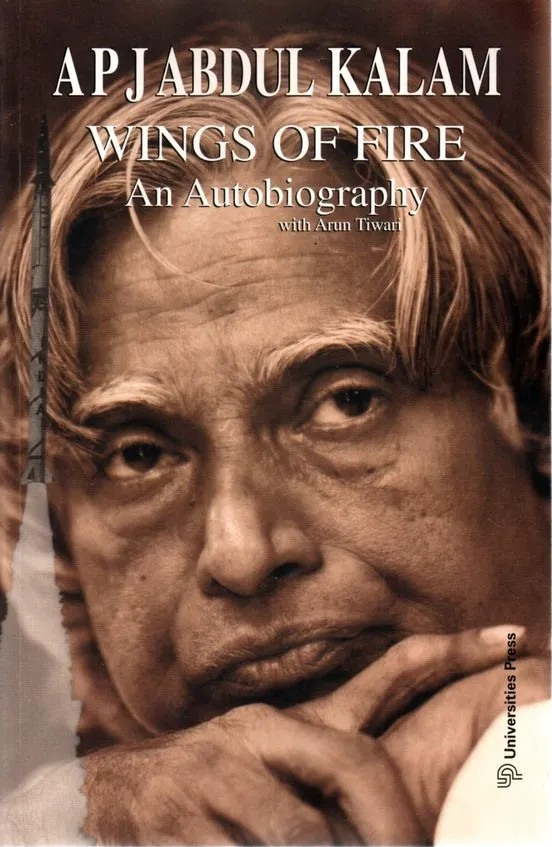
\includegraphics[width=0.45\textwidth,height=\textheight]{images/Wings-of-Fire.jpg}
\caption{\emph{Wings of Fire}.}
\end{figure}

\hypertarget{a-quote-to-ponder-on}{%
\subsection{A quote to ponder on}\label{a-quote-to-ponder-on}}

Part of the above quote encapsulates a little known truth about a law of
human consciousness, and bears repeated reading so that its full import
may be imbibed gradually. I repeat it below:

\begin{quote}
``Desire, when it stems from the heart and spirit, when it is pure and
intense, possesses awesome electromagnetic energy. This energy is
released into the ether each night, as the mind falls into the sleep
state. Each morning it returns to the conscious state reinforced with
the cosmic currents. That which has been imaged will surely and
certainly be manifested. You can rely, young man, upon this ageless
promise as surely as you can rely upon the eternally unbroken promise of
sunrise\ldots{} and of Spring.''
\end{quote}

While we have no scientific studies---according to the prevailing
\href{https://dictionary.cambridge.org/dictionary/english/double-blind}{double-blind}
orthodoxy---to uphold the veracity of the above statement, there has
been a steady procession of books of the ``manifesting'' genre
\protect\hyperlink{ref-murphy2006}{{[}3{]}}--\protect\hyperlink{ref-ferraro2021}{{[}8{]}}
which deal with actualizing your desires or dreams. It is astounding
that Swami Sivananda used the word ``manifested'' decades before the
advent of books like these.

\hypertarget{fulfilment-of-the-desire-to-fly}{%
\subsection{Fulfilment of the desire to
fly}\label{fulfilment-of-the-desire-to-fly}}

After Dr Abdul Kalam became President of India, he \emph{did get} an
opportunity both to learn flying, and to pilot a fighter jet. He
describes it himself
\href{https://www.youtube.com/shorts/kWnxd3af4rM}{in this short YouTube
video}. It is heartwarming to hear him explain how his desire to be a
pilot was ultimately fulfilled. \emph{This is anecdotal evidence that
this law of consciousness really works.}

\hypertarget{neville-goddards-feeling-is-the-secret}{%
\subsection{\texorpdfstring{Neville Goddard's \emph{Feeling Is the
Secret}}{Neville Goddard's Feeling Is the Secret}}\label{neville-goddards-feeling-is-the-secret}}

In 1944, a book was published bearing the title \emph{Feeling Is the
Secret}, by \href{feeling\%20is\%20the\%20secret}{Neville Goddard}. I
like it most among all the books of the ``manifesting'' genre because it
is clear, succinct, precise, and algorithmic. It provides a step-by-step
method to implement the technique alluded to by Swami Sivananda, with
very little filler material.

Fortunately for us,
\href{https://www.youtube.com/watch?v=ffNWoefuwPM}{the book is available
on YouTube} where a gentleman reads out the text at a decent pace. The
distinctive feature of this presentation is that the book's pages are
also clearly visible for us to read along as we hear the video
presentation.

\begin{figure}
\centering
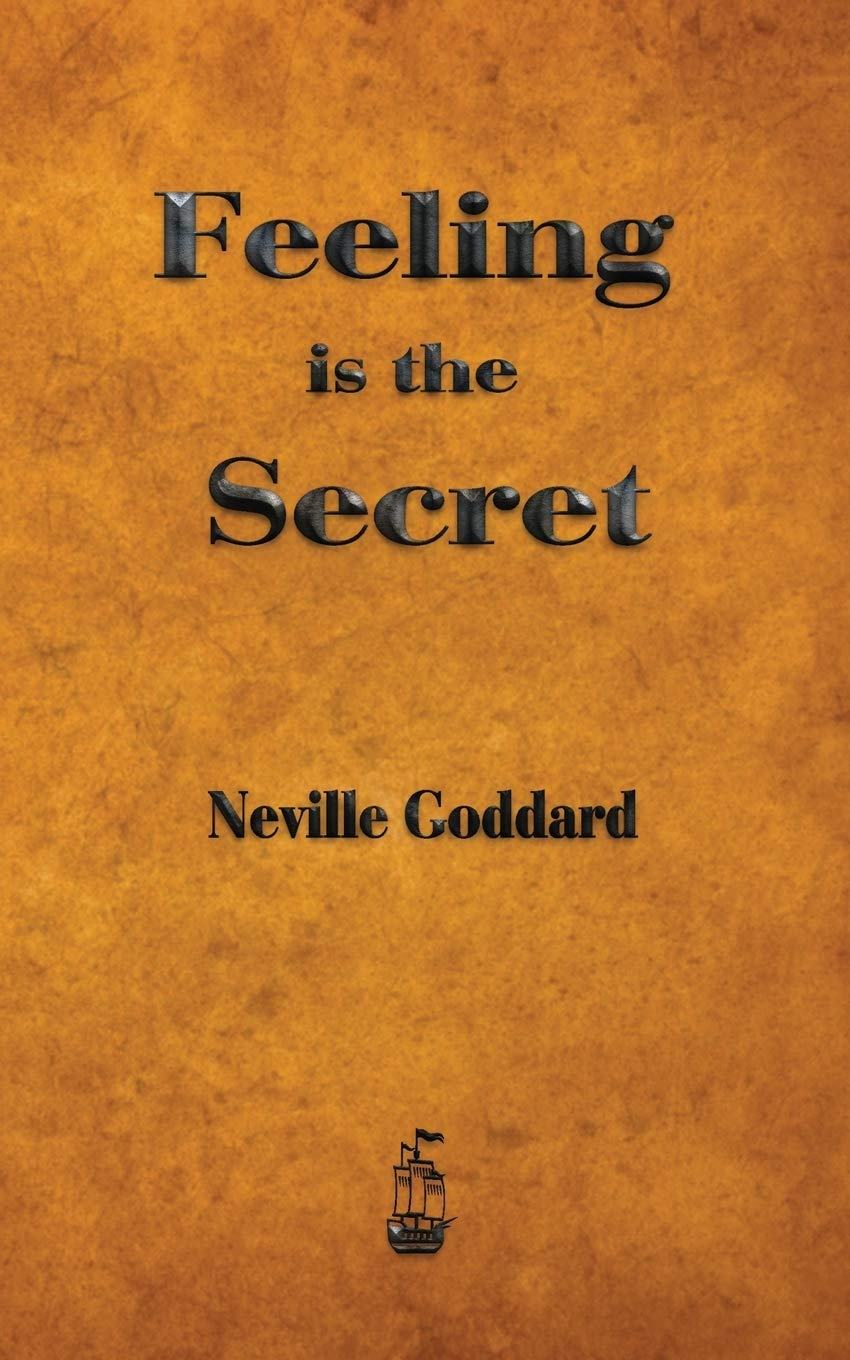
\includegraphics[width=0.45\textwidth,height=\textheight]{images/Feeling-is-the-Secret.jpg}
\caption{\emph{Feeling Is the Secret}.}
\end{figure}

Because the book is short---at 53 pages, and is less than forty minutes
long when heard as audio---it is ideal for each person to distil the
book into an algorithm that they can use for their entire life. This law
of consciousness may be used by each person to manifest his or her
personal desires. The only caveat is that one's intentions should be
clear, whole-hearted, noble, pure, and sincere.

yad bhāvaṃ tad bhavati.

यद् भावं तद् भवति ।

As you feel, so you become.

Happy manifesting!

\hypertarget{acknowledgements}{%
\subsection{Acknowledgements}\label{acknowledgements}}

I am grateful to Mr Phani Praveen for bringing to my attention the
\href{https://www.youtube.com/shorts/kWnxd3af4rM}{short YouTube video}
wherein Dr Abdul Kalam explains how his desire to be a pilot was
ultimately fulfilled.

\hypertarget{feedback}{%
\subsection{Feedback}\label{feedback}}

Please \href{mailto:feedback.swanlotus@gmail.com}{email me} your
comments and corrections.

\noindent A PDF version of this article is
\href{./feeling.pdf}{available for download here}:

\begin{normalsize}

\begin{ttfamily}

\url{https://swanlotus.netlify.app/blogs/feeling.pdf}

\end{ttfamily}

\end{normalsize}

\hypertarget{bibliography}{%
\section*{References}\label{bibliography}}
\addcontentsline{toc}{section}{References}

\hypertarget{refs}{}
\begin{CSLReferences}{0}{0}
\leavevmode\vadjust pre{\hypertarget{ref-kalam-wof-1999}{}}%
\CSLLeftMargin{{[}1{]} }%
\CSLRightInline{APJ Abdul Kalam and A Tiwari, \emph{{Wings of Fire: An
Autobiography}}. Universities Press, 1999. }

\leavevmode\vadjust pre{\hypertarget{ref-kalam-wof-online}{}}%
\CSLLeftMargin{{[}2{]} }%
\CSLRightInline{APJ Abdul Kalam and A Tiwari, {`{Wings of Fire: An
Autobiography}'}, 2016. {[}Online{]}. Available:
\url{https://ati.dae.gov.in/ati12052021_8.pdf}. {[}Accessed:
29-Jan-2023{]}}

\leavevmode\vadjust pre{\hypertarget{ref-murphy2006}{}}%
\CSLLeftMargin{{[}3{]} }%
\CSLRightInline{J. Murphy, \emph{The power of your subconscious mind}.
Pocket Books, 1997. }

\leavevmode\vadjust pre{\hypertarget{ref-hill1928}{}}%
\CSLLeftMargin{{[}4{]} }%
\CSLRightInline{N. Hill, \emph{The law of success: In sixteen lessons}.
Meriden, CT, USA: The Ralston University Press, 1928. }

\leavevmode\vadjust pre{\hypertarget{ref-byrne2006}{}}%
\CSLLeftMargin{{[}5{]} }%
\CSLRightInline{R. Byrne, \emph{The secret}. Atria Books, Beyond Words
Publishing, 2006. }

\leavevmode\vadjust pre{\hypertarget{ref-goddard2013}{}}%
\CSLLeftMargin{{[}6{]} }%
\CSLRightInline{N. Goddard, \emph{Feeling is the secret}. Merchant
Books, 2013. }

\leavevmode\vadjust pre{\hypertarget{ref-hicks2022}{}}%
\CSLLeftMargin{{[}7{]} }%
\CSLRightInline{E. Hicks and J. Hicks, \emph{Ask and it is given:
Learning to manifest your desires}. Hay House India, 2022. }

\leavevmode\vadjust pre{\hypertarget{ref-ferraro2021}{}}%
\CSLLeftMargin{{[}8{]} }%
\CSLRightInline{K. Ferraro, \emph{Manifesting}. St. Martin's Essentials,
2021. }

\end{CSLReferences}



\end{document}
